\documentclass[conference]{IEEEtran}
\IEEEoverridecommandlockouts
\usepackage{cite}
\usepackage{amsmath,amssymb}
\usepackage{graphicx}
\usepackage{booktabs}
\usepackage{multirow}
\usepackage{algorithm}
\usepackage{algpseudocode}
\usepackage{tikz}
\usetikzlibrary{arrows.meta,positioning,fit,calc}
\usepackage{xcolor}
\usepackage{url}
\usepackage[hidelinks]{hyperref}
\graphicspath{{figures/}}

\begin{document}

\title{TrialMatch: Criterion-Level Clinical Trial Eligibility Screening with a Fine-Tuned Open Transformer, Explicit KV Caching, Tiled Attention and Speculative Decoding}

\author{\IEEEauthorblockN{Fatima Farrukh Rana}
\IEEEauthorblockA{Roll No.\ 23i-0773, Generative AI (Assignment 2)\\
FAST National University of Computer and Emerging Sciences, Islamabad, Pakistan\\
fatimafarrukhfyp@gmail.com}}

\maketitle

\begin{abstract}
Screening a patient against every inclusion and exclusion criterion of a clinical trial is slow manual work, and an automated assistant is only useful if each decision is traceable to the patient record. We fine-tune Qwen2.5-1.5B-Instruct with LoRA on the TrialGPT Criterion Annotations dataset, using a fixed patient-grouped 37/8/8 split, so that it maps a patient note, a criterion type and a criterion text to a structured JSON answer: an eligibility label from the dataset's own label set and the IDs of the supporting note sentences. On the 206 held-out test criteria of 8 unseen patients, fine-tuning raises accuracy from 0.180 to 0.694, macro-F1 from 0.164 to 0.420 and evidence-sentence micro-F1 from 0.221 to 0.510, with 100\% parseable outputs. Error analysis shows that the remaining errors concentrate in rare labels and in exclusion criteria, where the model reproduces the dataset's convention of treating unmentioned conditions as absent. We also implement, from model forward passes upward, a hand-written decoder with an explicit key/value cache (token-identical to uncached decoding; 5.9$\times$ faster at 1024 input tokens on a T4), a tiled online-softmax attention (maximum error $2.3\times10^{-6}$ in fp32 and 59$\times$ less memory than the reference at 4096 tokens) and greedy speculative decoding with a 0.5B draft (240/240 outputs identical to greedy; up to 98\% acceptance, but 0.58--1.02$\times$ speed at batch size 1, which we explain). All components are exposed in a browser application that produces an evidence-linked, exportable screening report.
\end{abstract}

\begin{IEEEkeywords}
clinical trial matching, eligibility criteria, large language models, LoRA, KV cache, online softmax, speculative decoding
\end{IEEEkeywords}

% =====================================================================
\section{Introduction}
Clinical trials recruit poorly: many fail to enrol enough participants, and checking a candidate against tens of free-text criteria is done by hand. Large language models (LLMs) can read both the patient record and the criteria, and TrialGPT~\cite{trialgpt} showed that GPT-4 can predict criterion-level eligibility and cite evidence sentences. Two practical problems remain. First, a proprietary API is often unacceptable for patient data and cannot be inspected; second, a model that answers without pointing at the record cannot be audited.

\textbf{Problem statement.} Given (i) a patient note split into numbered sentences, (ii) a criterion type (inclusion or exclusion) and (iii) a criterion text, predict the criterion-level label used by the expert annotators---\emph{included}, \emph{not included}, \emph{not enough information} or \emph{not applicable} for inclusion criteria and \emph{excluded}, \emph{not excluded}, \emph{not enough information} or \emph{not applicable} for exclusion criteria---and return the IDs of the note sentences that support the decision. Absence of evidence must never be treated as proof of eligibility or ineligibility.

\textbf{Contributions.} (1) A reproducible LoRA fine-tune of an open 1.5B decoder on the prescribed split, with a before/after comparison on identical examples and an honest error analysis. (2) A hand-written Qwen2 forward pass with an explicit, preallocated KV cache, verified token-by-token against uncached decoding and Hugging Face \texttt{generate}. (3) A tiled online-softmax attention validated against a float64 reference. (4) Greedy speculative decoding with explicit draft/target cache synchronisation. (5) A browser application exposing all of the above with an exportable, evidence-linked report. The system is an educational screening prototype, not a clinical enrolment tool.

% =====================================================================
\section{Related Work}
\textbf{Patient--trial matching.} Koopman and Zuccon~\cite{koopman} released the patient--trial test collection whose 2014/2015 TREC Clinical Decision Support topics are the patients in our data. Criteria2Query~\cite{criteria2query} parses criteria into structured database queries; it needs structured records and does not explain decisions against free-text notes. TrialGPT~\cite{trialgpt} uses GPT-4 to label each criterion and cite sentences, and its expert-annotated subset is the dataset we use. We study the same task with a 1.5B open model that runs on free hardware, and we never use TrialGPT's GPT-4 outputs as features or targets.

\textbf{Transformers and adaptation.} We build on the decoder-only Transformer~\cite{vaswani} as realised in Qwen2.5~\cite{qwen25}, which combines rotary position embeddings (RoPE)~\cite{rope} and grouped-query attention (GQA)~\cite{gqa}, a generalisation of multi-query attention~\cite{mqa}. Full fine-tuning of 1.5B parameters with Adam needs roughly 16 bytes per parameter (about 25\,GB), which exceeds a 15\,GB T4. LoRA~\cite{lora} trains low-rank updates to frozen weights; QLoRA~\cite{qlora} additionally quantises the frozen base to 4 bits. Because the 1.5B base already fits in fp16 (3.1\,GB), we chose plain LoRA and avoided quantisation error and the \texttt{bitsandbytes} dependency.

\textbf{Efficient inference.} KV caching is the standard way to avoid recomputing keys and values during autoregressive decoding; Pope et al.~\cite{pope} analyse its memory cost, and PagedAttention~\cite{vllm} manages it in pages for serving. Rabe and Staats~\cite{rabe} showed that attention can be computed in chunks with constant memory per query, and FlashAttention~\cite{flashattn} computes exact attention in tiles using the online softmax of Milakov and Gimelshein~\cite{onlinesoftmax}, never materialising the full score matrix. Speculative decoding~\cite{leviathan,chen} lets a small draft model propose tokens that the target verifies in one pass; with greedy acceptance the output is provably identical to the target's greedy decoding. Its benefit depends on the draft's relative cost and acceptance rate, which we measure rather than assume.

% =====================================================================
\section{Materials and Methods}

\subsection{Dataset, Split and Leakage Control}
The TrialGPT Criterion Annotations dataset~\cite{trialgptdata} has 1,015 criterion-level annotations covering 53 patients and 103 trials. Each row holds a patient note already split into numbered sentences (at most 14), the criterion type and text, the expert label and the expert evidence sentence IDs. Labels are imbalanced: \emph{not excluded} 484, \emph{not enough information} 293, \emph{included} 150, \emph{not applicable} 55, \emph{not included} 23, \emph{excluded} 10. 610 rows (60\%) have no expert evidence.

We keep only nine columns. All \texttt{gpt4\_*} columns, \texttt{explanation\_correctness} (an expert grade of GPT-4's explanation, which indirectly encodes GPT-4's output) and TrialGPT's own \texttt{training} flag are dropped before any processing. Annotation 883 has an empty criterion text and was removed (it would be a training row with no criterion to judge).

Following the protocol, unique patient IDs are sorted, shuffled with NumPy \texttt{default\_rng(42)}, and the first 37/next 8/last 8 patients form train/validation/test. This gives 602/206/206 annotations (Table~\ref{tab:split}). Every script re-derives the split, asserts that it equals the published manifest, and checks that no patient appears in two splits; we additionally verified that no identical note and no identical (note, criterion) pair occurs in more than one split. The test split contains no \emph{excluded} example, so test macro-F1 averages over the five labels present. The test split was evaluated exactly once, after all choices were frozen on validation.

\begin{table}[t]
\centering
\caption{Patient-grouped split (seed 42) and expert label distribution.}
\label{tab:split}
\footnotesize
\resizebox{\columnwidth}{!}{%
\begin{tabular}{lccc}
\toprule
 & Train & Validation & Test \\
\midrule
Patients / trials & 37 / 72 & 8 / 16 & 8 / 16 \\
Annotations (incl. / excl.) & 602 (215 / 387) & 206 (66 / 140) & 206 (75 / 131) \\
\midrule
included & 88 & 35 & 27 \\
not included & 13 & 3 & 7 \\
excluded & 8 & 2 & 0 \\
not excluded & 291 & 101 & 91 \\
not enough information & 174 & 53 & 66 \\
not applicable & 28 & 12 & 15 \\
\midrule
No gold evidence & 348 & 116 & 145 \\
Prompt tokens (mean / max) & 355 / 636 & 368 / 476 & 338 / 540 \\

\bottomrule
\end{tabular}}
\end{table}

\subsection{Model Selection}
Table~\ref{tab:models} compares the candidates. We needed a decoder-only model with a chat template, a permissive licence, a fine-tune that fits a free 15\,GB T4, and a smaller sibling with the \emph{same tokenizer} for speculative decoding.

\begin{table}[t]
\centering
\caption{Open-weight decoder candidates (official model cards). KV = 16-bit key/value cache per 1,000 tokens.}
\label{tab:models}
\resizebox{\columnwidth}{!}{%
\begin{tabular}{lccccl}
\toprule
Model & Params & Layers / heads (KV) & Context & KV (MB) & Licence \\
\midrule
\textbf{Qwen2.5-1.5B-Instruct} & 1.54B & 28 / 12 (2) & 32K & 28.7 & Apache-2.0 \\
Qwen2.5-0.5B-Instruct (draft) & 0.49B & 24 / 14 (2) & 32K & 12.3 & Apache-2.0 \\
Llama-3.2-1B-Instruct & 1.24B & 16 / 32 (8) & 128K & 32.8 & Llama 3.2 (gated) \\
SmolLM2-1.7B-Instruct & 1.71B & 24 / 32 (32) & 8K & 196.6 & Apache-2.0 \\
Phi-3.5-mini-instruct & 3.8B & 32 / 32 (32) & 128K & 393.2 & MIT \\
\bottomrule
\end{tabular}}
\end{table}

Qwen2.5-1.5B-Instruct was selected because (i) its fp16 weights (3.1\,GB) plus LoRA training fit a T4 with room for activations (measured peak 8.5\,GB); (ii) GQA with only 2 KV heads makes the cache small, $2 \cdot 28 \cdot 2 \cdot 128 \cdot 2 = 28{,}672$ bytes per token in fp16; (iii) Qwen2.5-0.5B-Instruct (494M parameters, 24 layers, 14 heads, 2 KV heads) shares the exact 151,665-token vocabulary, which speculative decoding requires (we assert vocabulary equality in code); and (iv) Apache-2.0 permits redistribution of adapters. Llama-3.2-1B is gated by a custom licence and its draft sibling is not smaller; SmolLM2 uses full multi-head attention (about 7$\times$ more KV memory per token than Qwen) and an 8K context; Phi-3.5-mini (3.8B) would require 4-bit quantisation to fine-tune on a T4.

\subsection{Input/Output Format and Tokenisation}
The prompt is built with Qwen's chat template: a system message (``judge one criterion against one note using only what the note says; absence of a statement is not proof either way''), then the numbered note, the criterion type, the criterion text, the four labels allowed for that type with one-line definitions, and the output instruction. The target is a single JSON object with the evidence first, so that the label is generated after the cited sentences:
\begin{center}\small\texttt{\{"evidence": [0, 3], "label": "not included"\}}\end{center}
The dataset contains no expert-written explanations (only GPT-4's, which we may not use), so the model is not trained to explain. Explanations shown to users are templates filled only from the predicted label and the quoted cited sentences, which makes them faithful by construction.

With the Qwen2.5 BPE tokenizer, prompts are 267--636 tokens (mean 354, 95th percentile 497) and targets 13--39 tokens. The longest training sequence is 663 tokens, far below both the 1,536-token limit we set and the 32K context, so \textbf{no example is truncated and no evidence is lost}; the training script raises an error rather than truncating silently.

\subsection{Fine-Tuning}
We train LoRA adapters ($r{=}16$, $\alpha{=}32$, dropout 0.05) on all attention and MLP projections (q, k, v, o, gate, up, down): 18.5M trainable parameters, 1.2\% of the model. The objective is next-token cross-entropy on the assistant's JSON only; all prompt tokens are masked with $-100$. Training uses AdamW~\cite{adamw} at learning rate $2\times10^{-4}$ with cosine decay and 10 warm-up steps, effective batch 16 (4$\times$4 accumulation), 3 epochs (114 steps), fp16 mixed precision with fp32 adapter weights, and gradient checkpointing. The checkpoint with the lowest validation loss is kept. One run takes 16.3 minutes on a free Colab T4.

\subsection{System Architecture}
Fig.~\ref{fig:arch} shows the pipeline used by both evaluation and the application.

\begin{figure*}[t]
\centering
\begin{tikzpicture}[font=\footnotesize,
  box/.style={draw, rounded corners=2pt, fill=blue!6, align=center, text width=2.6cm, minimum height=9mm, inner sep=2pt},
  model/.style={draw, rounded corners=2pt, fill=orange!12, align=center, text width=3.3cm, minimum height=9mm, inner sep=2pt},
  out/.style={draw, rounded corners=2pt, fill=green!8, align=center, text width=2.8cm, minimum height=9mm, inner sep=2pt},
  arr/.style={-{Stealth[length=2mm]}, thick}]
\node[box]   (note)   at (0,0.75)   {Patient note (free text or numbered)};
\node[box]   (crit)   at (0,-0.75)  {Criteria text or ClinicalTrials.gov ID};
\node[box]   (split)  at (3.3,0.75) {Sentence splitter (IDs 0..n)};
\node[box]   (parse)  at (3.3,-0.75){Criterion parser (type + text)};
\node[box]   (prompt) at (6.6,0)    {Prompt builder: chat template, allowed labels};
\node[model] (dec)    at (10.3,0)   {Qwen2.5-1.5B + LoRA, hand-written decoder (KV cache, RoPE, GQA)};
\node[model] (draft)  at (10.3,1.65){0.5B draft (speculative)};
\node[model] (attn)   at (10.3,-1.65){Attention: SDPA / reference / tiled};
\node[out]   (json)   at (14.2,0)   {JSON \{evidence, label\}: parser + ID check};
\node[out]   (expl)   at (14.2,1.65){Evidence text + template explanation};
\node[out]   (agg)    at (14.2,-1.65){Rule-based overall outcome};
\node[out]   (rep)    at (14.2,-3.05){HTML / JSON report with provenance};
\draw[arr] (note) -- (split); \draw[arr] (crit) -- (parse);
\draw[arr] (split) -- (prompt); \draw[arr] (parse) -- (prompt);
\draw[arr] (prompt) -- (dec); \draw[arr] (draft) -- node[right, font=\scriptsize]{propose $k$} (dec);
\draw[arr] (attn) -- (dec); \draw[arr] (dec) -- (json);
\draw[arr] (json) -- (expl); \draw[arr] (json) -- (agg); \draw[arr] (agg) -- (rep);
\end{tikzpicture}
\caption{TrialMatch pipeline. The same prompt builder, decoder and parser are used for offline evaluation and in the browser application. Orange: Transformer components implemented in this work.}
\label{fig:arch}
\end{figure*}

\subsection{KV-Cached Decoding (Task 3)}
We do not call \texttt{generate(use\_cache=True)}. \texttt{ManualQwen2} uses the Hugging Face Transformers~\cite{hftransformers} model only as a container of weights (embedding, linear layers, RMSNorm) and implements RoPE, grouped-query attention, the causal mask, the residual stream and the cache itself. The cache holds, per layer, preallocated tensors $K,V\in\mathbb{R}^{B\times h_{kv}\times L_{\max}\times d}$ and a length counter $\ell$ (Fig.~\ref{fig:decoder}, Algorithm~\ref{alg:kv}).

\textbf{Positional handling.} New tokens receive absolute positions $\ell,\dots,\ell+T-1$. RoPE is applied to $q$ and $k$ (never $v$) \emph{before} $k$ is written, so cached keys already carry their rotation and are never re-rotated.
\textbf{Masking.} A query at absolute position $p$ may attend to keys $0..p$. Because the queries of a chunk start at offset $\ell$, key $j$ is masked when $j > \ell+i$; PyTorch's \texttt{is\_causal=True} aligns the triangle top-left and would be wrong for any chunk that starts after position 0, so we pass the offset mask explicitly. For a single decode token no key is masked.
\textbf{Cache growth.} Memory is allocated once for prompt length plus the token budget; each step writes one slot per layer. Memory grows linearly (28\,KB/token for the 1.5B model) instead of the quadratic recomputation of the uncached path. A \texttt{crop}($n$) operation rolls the cache back, which speculative decoding uses.
\textbf{Shared-prefix reuse.} In the application all criteria of one patient share the system prompt and note; we prefill that prefix once and crop back to it before each criterion, which gives identical outputs while skipping 221--234 prefix tokens per criterion.

\begin{figure}[t]
\centering
\resizebox{0.95\columnwidth}{!}{%
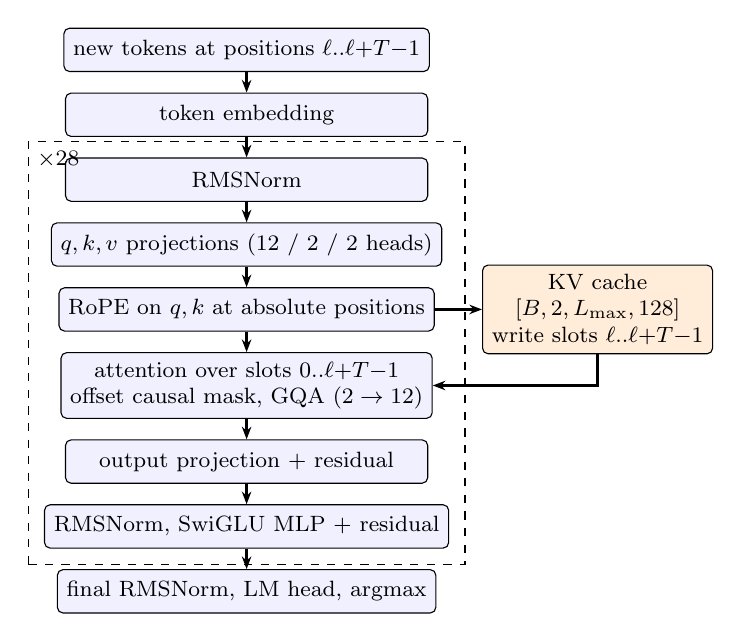
\begin{tikzpicture}[font=\footnotesize, node distance=2.6mm,
  st/.style={draw, rounded corners=2pt, fill=blue!6, minimum width=46mm, minimum height=5.5mm, align=center},
  kv/.style={draw, rounded corners=2pt, fill=orange!15, align=center, minimum height=10mm},
  arr/.style={-{Stealth[length=1.6mm]}, thick}]
\node[st] (in) {new tokens at positions $\ell..\ell{+}T{-}1$};
\node[st, below=of in] (emb) {token embedding};
\node[st, below=of emb] (n1) {RMSNorm};
\node[st, below=of n1] (qkv) {$q,k,v$ projections (12 / 2 / 2 heads)};
\node[st, below=of qkv] (rope) {RoPE on $q,k$ at absolute positions};
\node[st, below=of rope] (att) {attention over slots $0..\ell{+}T{-}1$\\offset causal mask, GQA ($2\rightarrow12$)};
\node[st, below=of att] (o) {output projection + residual};
\node[st, below=of o] (mlp) {RMSNorm, SwiGLU MLP + residual};
\node[st, below=of mlp] (head) {final RMSNorm, LM head, argmax};
\node[kv, right=6mm of rope] (cache) {KV cache\\$[B,2,L_{\max},128]$\\write slots $\ell..\ell{+}T{-}1$};
\node[draw, dashed, fit=(n1)(mlp), inner sep=2mm, label={[anchor=north west]north west:{$\times28$}}] {};
\foreach \a/\b in {in/emb,emb/n1,n1/qkv,qkv/rope,rope/att,att/o,o/mlp,mlp/head} \draw[arr] (\a) -- (\b);
\draw[arr] (rope.east) -- (cache.west);
\draw[arr] (cache.south) |- (att.east);
\end{tikzpicture}}
\caption{One forward step of the hand-written Qwen2.5 decoder. Keys are cached after RoPE, so they are never re-rotated; attention reads all cached positions plus the new ones.}
\label{fig:decoder}
\end{figure}

\begin{algorithm}[t]
\caption{Greedy decoding with an explicit KV cache}\label{alg:kv}
\small
\begin{algorithmic}[1]
\State $C \gets$ empty cache with $L_{\max}=|x|+N$; $\ell\gets0$
\State $z \gets \textsc{Forward}(x_{0..|x|-1}, \text{pos}=0..|x|-1, C)$ \Comment{prefill, writes $K,V$}
\State $y_1 \gets \arg\max z_{\text{last}}$; $\ell \gets |x|$
\For{$t=2..N$ \textbf{while} $y_{t-1}\neq\text{EOS}$}
  \State $z \gets \textsc{Forward}(y_{t-1}, \text{pos}=\ell, C)$ \Comment{1 query, attends to $K_{0..\ell}$}
  \State $y_t \gets \arg\max z$; $\ell \gets \ell+1$
\EndFor
\end{algorithmic}
\end{algorithm}

\subsection{Tiled Online-Softmax Attention (Task 4)}
The reference computes $\mathrm{softmax}(QK^\top/\sqrt{d}+M)V$ in fp32 after subtracting each row's maximum, materialising the $T_q\times T_k$ matrix. The tiled version (Algorithm~\ref{alg:tiled}) processes query blocks and, inside each, key/value blocks, keeping a running maximum $m$, normaliser $l$ and unnormalised output $a$ per query, so memory is $O(B_q\cdot B_k)$ per tile instead of $O(T^2)$. Key blocks entirely in a query block's future are skipped, and rows whose keys are all masked so far use 0 in place of $-\infty$ in the exponent to avoid NaN. No fused backend is called.

\begin{algorithm}[t]
\caption{Tiled attention with online softmax (one query block)}\label{alg:tiled}
\small
\begin{algorithmic}[1]
\State $m\gets-\infty$, $l\gets0$, $a\gets0$ \Comment{per query row}
\For{each key block $(K_j, V_j)$ not entirely in the future}
  \State $S \gets Q_b K_j^\top/\sqrt{d}$; apply offset causal mask
  \State $m' \gets \max(m, \text{rowmax}(S))$; $\alpha\gets e^{m-m'}$; $P\gets e^{S-m'}$
  \State $l \gets \alpha l + \text{rowsum}(P)$; $a \gets \alpha a + P V_j$; $m\gets m'$
\EndFor
\State \Return $a / l$
\end{algorithmic}
\end{algorithm}

\subsection{Greedy Speculative Decoding (Task 5)}
The target (fine-tuned 1.5B) and the draft (0.5B) each run through \texttt{ManualQwen2} with their own cache. Between rounds, the last committed token $x$ is \emph{pending}: produced by the target but in neither cache. One round (Algorithm~\ref{alg:spec}) drafts $k$ tokens, verifies all of them with one target forward over $k{+}1$ tokens, accepts the longest matching prefix and appends the target's own next token (a correction on rejection, a free bonus token when all $k$ are accepted). Both caches are then cropped to the committed prefix; after a fully accepted round the draft lags one token and feeds two tokens next round. Every committed token is the target's greedy choice given the committed prefix, so the output equals target greedy decoding up to floating-point effects.

\begin{algorithm}[t]
\caption{One round of greedy speculative decoding}\label{alg:spec}
\small
\begin{algorithmic}[1]
\State $d_1..d_k \gets$ draft greedily continues $\text{seq}[\ell_D:]$ \Comment{$k$ small forwards}
\State $p_0..p_k \gets \arg\max \textsc{Target}([x, d_1..d_k])$ \Comment{one forward}
\State $n \gets \max\{n: d_i = p_{i-1}\ \forall i\le n\}$
\State commit $d_1..d_n, p_n$; \textsc{Crop}$(C_T, |\text{seq}|_{\text{old}}+n)$; \textsc{Crop}$(C_D, \min(\ell_D, |\text{seq}|_{\text{old}}+n))$
\end{algorithmic}
\end{algorithm}

The draft is Qwen2.5-0.5B-Instruct; we compare its base version with a version fine-tuned with the same recipe (best validation loss 0.134). Both models in fp16 use 4.1\,GB, well within the T4.

\subsection{Browser Application (Task 6)}
A Gradio application (Fig.~\ref{fig:app}) accepts a free-text note (numbered automatically) and criteria typed, pasted or fetched by NCT ID from the public ClinicalTrials.gov API. The user picks the decoding mechanism (KV cache, speculative with draft length $k$, Hugging Face \texttt{generate}, or no cache). For each criterion it shows the label, the cited sentence IDs, highlighted evidence text and the template explanation; it lists criteria with missing information and decisive labels without cited evidence, and it reports a preliminary overall outcome from explicit rules: any inclusion \emph{not included} or exclusion \emph{excluded} gives \emph{likely ineligible}; otherwise any \emph{not enough information} gives \emph{undetermined}; otherwise \emph{potentially eligible}; \emph{not applicable} is ignored. This outcome is labelled as an aggregation, not a ground-truth label. Reports download as HTML and JSON with provenance (model, adapter, decoding mode, device, dtype, code commit, input hash, timestamp). An \emph{Inference comparison} tab runs one criterion through the selected mechanisms live and checks token equality; a live attention check compares the three attention implementations against float64. Invalid inputs (Fig.~\ref{fig:validation}; empty note, no criteria, over-long notes, malformed NCT IDs, insufficient memory for the draft) produce readable errors. The application starts with one command (\texttt{./run\_app.sh}), chooses fp32 on CPU when memory allows (bf16 otherwise) and fp16 on GPU.

\begin{figure*}[!t]
\centering
\begin{minipage}[t]{0.49\textwidth}\centering
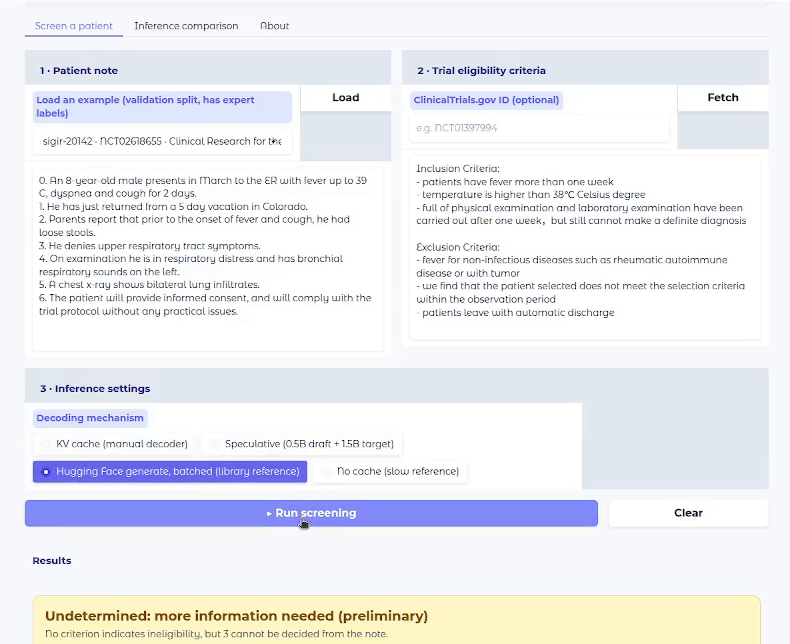
\includegraphics[width=\linewidth]{app_input.png}\\[-1mm]
{\footnotesize (a) Input: patient note, criteria (typed, pasted or fetched by NCT ID), decoding mechanism.}
\end{minipage}\hfill
\begin{minipage}[t]{0.49\textwidth}\centering
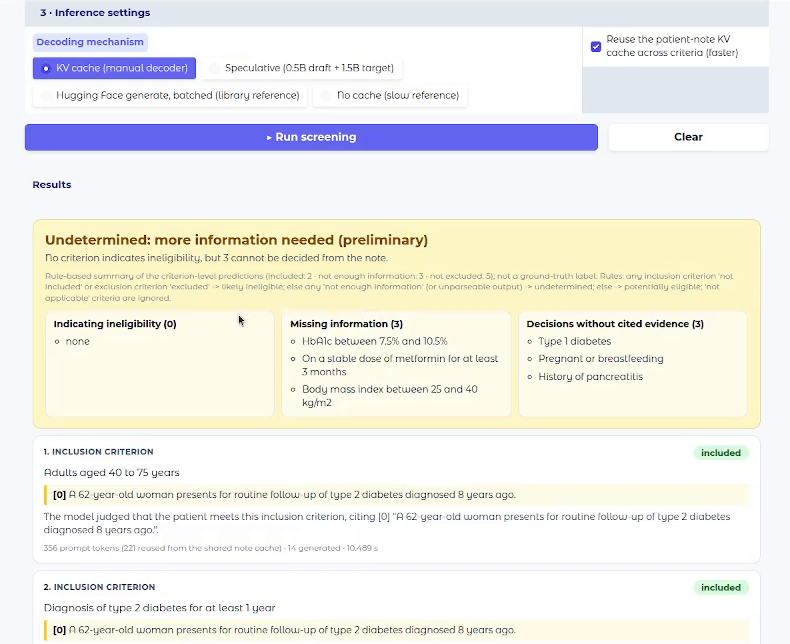
\includegraphics[width=\linewidth]{app_results.png}\\[-1mm]
{\footnotesize (b) Unseen diabetes case: rule-based outcome, missing information, decisions without evidence, evidence-linked criterion cards.}
\end{minipage}\\[3mm]
\begin{minipage}[t]{0.49\textwidth}\centering
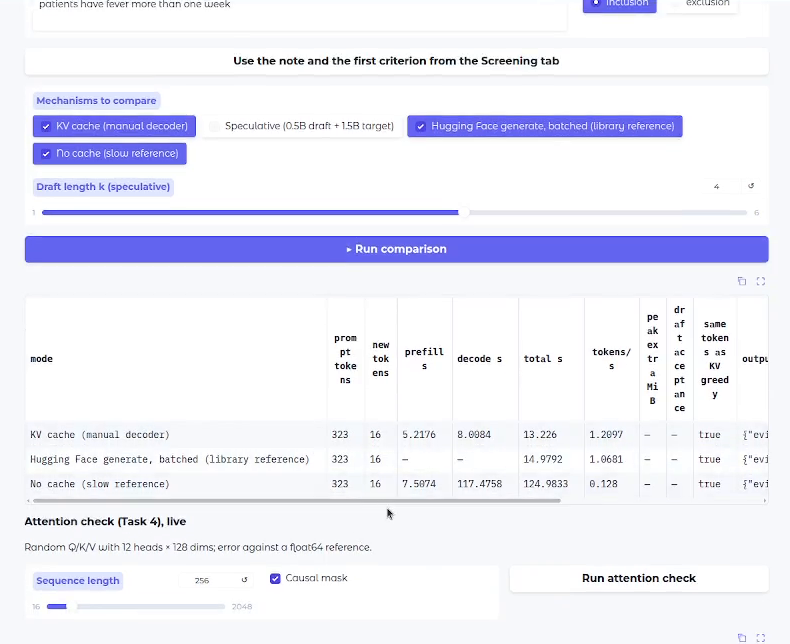
\includegraphics[width=\linewidth]{app_compare.png}\\[-1mm]
{\footnotesize (c) Live inference comparison: identical tokens for KV-cache, Hugging Face and no-cache decoding (13.2\,s vs.\ 125.0\,s on CPU).}
\end{minipage}\hfill
\begin{minipage}[t]{0.49\textwidth}\centering
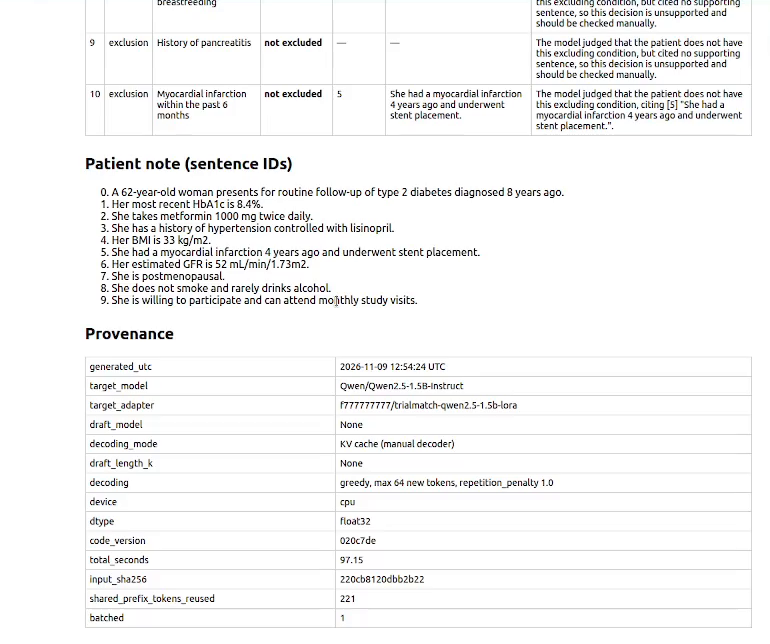
\includegraphics[width=\linewidth]{app_report.png}\\[-1mm]
{\footnotesize (d) Exported HTML report: cited evidence, numbered note and provenance (model, adapter, mode, dtype, commit, input hash).}
\end{minipage}
\caption{TrialMatch browser application on a laptop CPU (fp32, fine-tuned adapter loaded).}
\label{fig:app}
\end{figure*}

\begin{figure}[t]
\centering
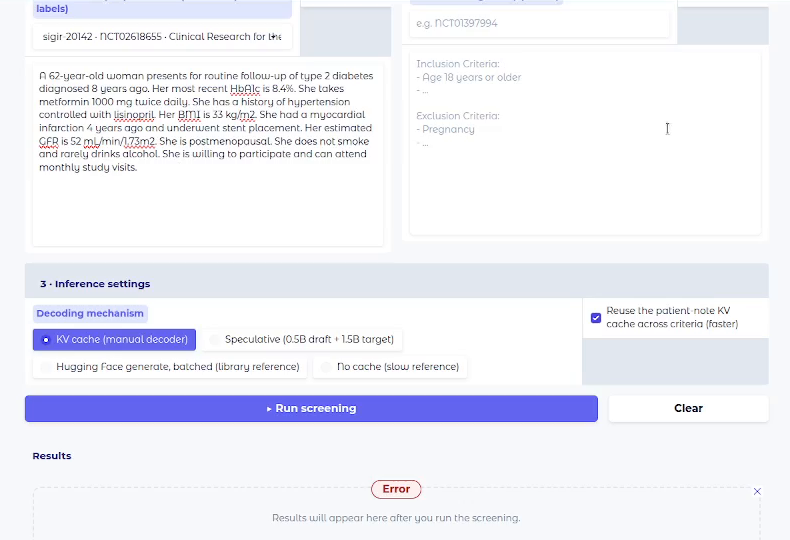
\includegraphics[width=0.9\columnwidth]{app_validation.png}
\caption{Recovery from invalid input: running without criteria shows a readable error and leaves the inputs intact.}
\label{fig:validation}
\end{figure}

% =====================================================================
\section{Experimental Setup and Metrics}
Training and all GPU benchmarks ran on a free Google Colab Tesla T4 (16\,GB, fp16, no bf16 or FlashAttention-2 support) with PyTorch 2.14 and Transformers 5.22; the application was additionally run on a laptop CPU (Intel i7-10610U, 4 cores, 15\,GB RAM). All decoding is deterministic greedy (\texttt{do\_sample=False}, one beam, repetition penalty 1.0, at most 64 new tokens); we replace Qwen's shipped generation configuration, which samples at temperature 0.7, so that results are reproducible and comparable.

\textbf{Classification.} Accuracy, macro-F1 (averaged over the labels present in the gold set of the evaluated split), per-class precision/recall/F1 and confusion matrices, overall and separately for inclusion and exclusion criteria. An output that cannot be parsed into an allowed label counts as wrong (none occurred).
\textbf{Evidence.} Sentence-ID retrieval is scored with \emph{micro} precision/recall/F1 pooled over all records (records with an empty gold set can only add false positives) and \emph{macro} averages over records with a non-empty gold set (an empty prediction there scores 0). For the 145 test records with no gold evidence we report separately how often the model also cites nothing.
\textbf{Baselines.} The same model zero-shot (identical prompt and decoding) and a majority-class baseline (the most frequent training label per criterion type).
\textbf{Inference benchmarks.} Each configuration runs once for warm-up and then 3 (KV) or 10 (attention) times with \texttt{torch.cuda.synchronize()} around each timed region; we report medians and peak memory above the loaded model.

% =====================================================================
\section{Results and Discussion}

\subsection{Fine-Tuning}
Fig.~\ref{fig:curves} shows that training loss falls from 0.57 to about 0.05, while validation loss reaches its minimum of 0.121 at step 50 (1.3 epochs) and then rises slightly. The model starts to memorise the 37 training patients after the first epoch, so the early checkpoint was kept.

\begin{figure}[t]
\centering
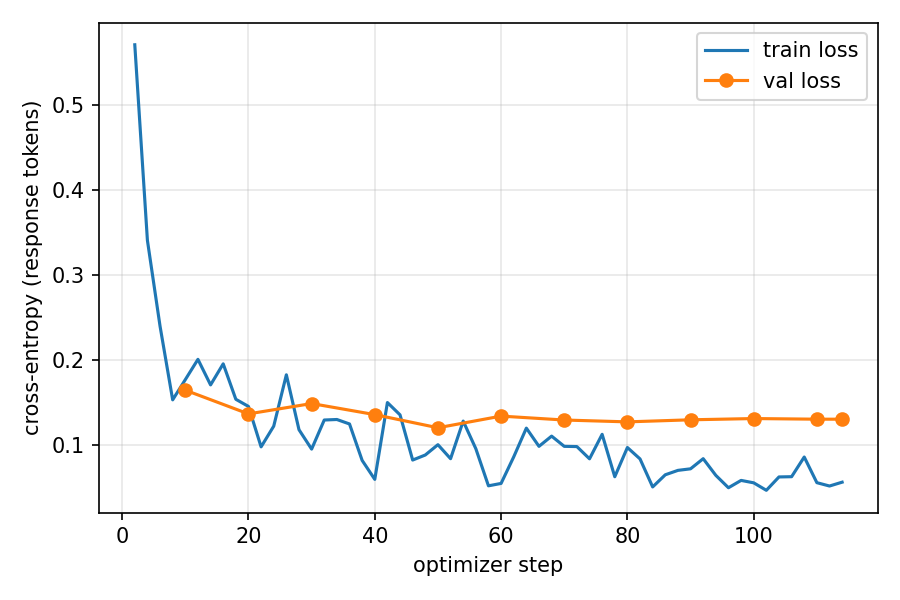
\includegraphics[width=0.49\columnwidth]{training_curves.png}\hfill
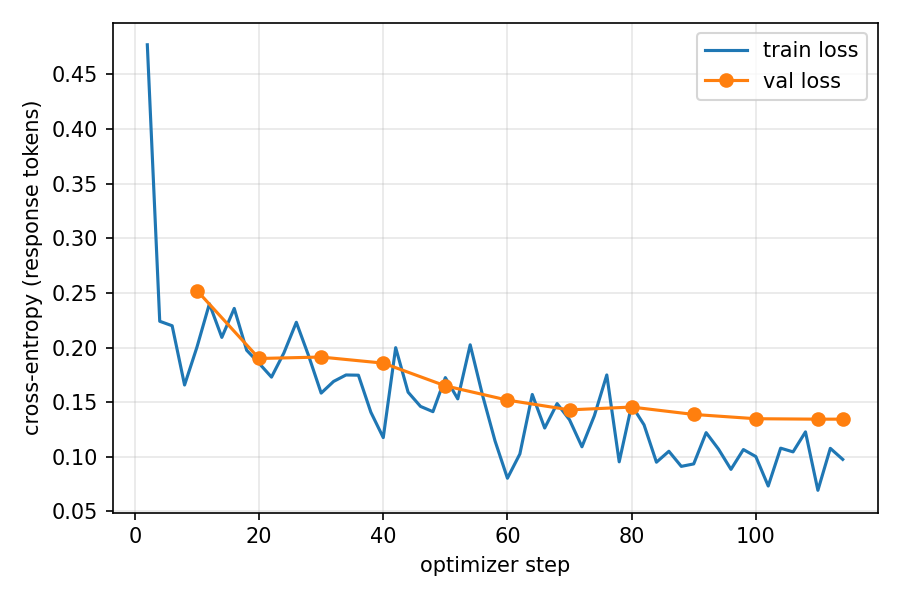
\includegraphics[width=0.49\columnwidth]{training_curves_draft05.png}
\caption{LoRA training curves (loss on response tokens). Left: 1.5B target, best validation loss at step 50 (used everywhere). Right: 0.5B draft, best at step 110.}
\label{fig:curves}
\end{figure}

\subsection{Before/After and Held-Out Results}
Table~\ref{tab:main} compares the same model before and after fine-tuning on identical validation and test examples. Zero-shot, the model produces valid JSON but over-uses \emph{not applicable} (88 of 91 \emph{not excluded} test cases) and cites many sentences, giving evidence precision of 0.15. Fine-tuning triples accuracy on both splits; test accuracy (0.694) equals validation accuracy, indicating no overfitting to the validation set used for checkpoint selection. Test macro-F1 is higher than validation macro-F1 (0.420 vs.\ 0.326) mainly because the test split has no \emph{excluded} class, so the average runs over five labels instead of six. On test, fine-tuning fixes 129 predictions and breaks 23 (validation: 128 and 29). Because annotations of one patient are correlated, we resampled whole patients (2,000 bootstrap draws of the 8 patients): the test accuracy gain is +0.52 (95\% CI 0.36--0.64) and the macro-F1 gain +0.26 (0.16--0.36); on validation +0.48 (0.31--0.62) and +0.16 (0.05--0.26). The fine-tuned test accuracy itself has a wide interval (0.55--0.81), a direct consequence of having only eight test patients. The zero-shot confusion matrix (Table~\ref{tab:cmbase}) shows why the base model fails: it answers \emph{not applicable} for 88 of the 91 \emph{not excluded} cases and never outputs \emph{not enough information}.

\begin{table*}[t]
\centering
\caption{Before/after fine-tuning (Qwen2.5-1.5B-Instruct, greedy, identical examples). The majority-class baseline on test scores accuracy 0.626, macro-F1 0.272 (inclusion 0.507, exclusion 0.695).}
\label{tab:main}
\begin{tabular}{llcccccc}
\toprule
Split & Model & Accuracy & Macro-F1 & Incl.\ acc. & Excl.\ acc. & Evidence micro-F1 & Evidence macro-F1 \\
\midrule
Val & Zero-shot & 0.214 & 0.171 & 0.439 & 0.107 & 0.195 & 0.204 \\
Val & LoRA & 0.694 & 0.326 & 0.636 & 0.721 & 0.570 & 0.575 \\
\midrule
Test & Zero-shot & 0.180 & 0.164 & 0.320 & 0.099 & 0.221 & 0.200 \\
Test & LoRA & 0.694 & 0.420 & 0.693 & 0.695 & 0.510 & 0.513 \\

\bottomrule
\end{tabular}
\end{table*}

The majority baseline is essential to read these numbers honestly. Overall, the fine-tuned model beats it (0.694 vs.\ 0.626 accuracy, 0.420 vs.\ 0.272 macro-F1), but on exclusion criteria it predicts \emph{not excluded} for all 131 test cases (Table~\ref{tab:cm}) and therefore only matches the baseline's 0.695. Its gains come from inclusion criteria (0.693 vs.\ 0.507) and from evidence retrieval, which the baseline cannot do at all. Per class (Table~\ref{tab:perclass}), \emph{included} predictions are always right (precision 1.00) but half of the true cases are called \emph{not enough information}, and the two rare labels present in test (\emph{not applicable}, \emph{not included}) are never predicted.

\begin{table}[t]
\centering
\caption{Per-class results on the test split (LoRA model; zero-shot F1 for reference).}
\label{tab:perclass}
\footnotesize
\begin{tabular}{lrcccc}
\toprule
Label & $n$ & F1 (zero-shot) & P & R & F1 \\
\midrule
included & 27 & 0.64 & 1.00 & 0.52 & 0.68 \\
not applicable & 15 & 0.16 & 0.00 & 0.00 & 0.00 \\
not enough information & 66 & 0.00 & 0.62 & 0.58 & 0.60 \\
not excluded & 91 & 0.02 & 0.69 & 1.00 & 0.82 \\
not included & 7 & 0.00 & 0.00 & 0.00 & 0.00 \\

\bottomrule
\end{tabular}
\end{table}

\begin{table}[t]
\centering
\caption{Zero-shot test confusion matrix, all 206 criteria (rows: expert label).}
\label{tab:cmbase}
\footnotesize
\resizebox{\columnwidth}{!}{\begin{tabular}{lrrrrrr}
\toprule
Gold $\downarrow$ / Pred $\rightarrow$ & incl. & N/A & NEI & not excl. & not incl. & excl. \\
\midrule
incl. & 22 & 5 & 0 & 0 & 0 & 0 \\
N/A & 1 & 14 & 0 & 0 & 0 & 0 \\
NEI & 13 & 50 & 0 & 2 & 0 & 1 \\
not excl. & 0 & 88 & 0 & 1 & 0 & 2 \\
not incl. & 6 & 1 & 0 & 0 & 0 & 0 \\
\bottomrule
\end{tabular}
}
\end{table}

\begin{table}[t]
\centering
\caption{Test confusion matrices of the LoRA model (rows: expert label).}
\label{tab:cm}
\footnotesize
\textbf{Inclusion criteria ($n{=}75$)}\\[1mm]
\begin{tabular}{lrrrr}
\toprule
Gold $\downarrow$ / Pred $\rightarrow$ & incl. & N/A & NEI & not incl. \\
\midrule
incl. & 14 & 0 & 13 & 0 \\
N/A & 0 & 0 & 3 & 0 \\
NEI & 0 & 0 & 38 & 0 \\
not incl. & 0 & 0 & 7 & 0 \\
\bottomrule
\end{tabular}
\\[2mm]
\textbf{Exclusion criteria ($n{=}131$)}\\[1mm]
\begin{tabular}{lrrr}
\toprule
Gold $\downarrow$ / Pred $\rightarrow$ & N/A & NEI & not excl. \\
\midrule
N/A & 0 & 0 & 12 \\
NEI & 0 & 0 & 28 \\
not excl. & 0 & 0 & 91 \\
\bottomrule
\end{tabular}

\end{table}

\subsection{Evidence Localisation}
Table~\ref{tab:evidence} shows that fine-tuning mainly improves precision: the model learns to cite one or two sentences instead of many (micro precision 0.15$\rightarrow$0.64) while keeping recall (0.43). For the 145 test records without gold evidence, the fine-tuned model also cites nothing 94\% of the time. Evidence is far better for inclusion (micro-F1 0.61) than for exclusion criteria (0.24), where most decisions are \emph{not excluded} with no citation. 115 of 206 test predictions have both the correct label and exactly the gold evidence set.

\begin{table}[t]
\centering
\caption{Evidence-sentence retrieval on the test split. ``Empty'' = share of records with no gold evidence for which the model also cites nothing.}
\label{tab:evidence}
\setlength{\tabcolsep}{2.5pt}
\footnotesize
\begin{tabular}{llccccccc}
\toprule
& & \multicolumn{3}{c}{Micro} & \multicolumn{3}{c}{Macro (gold $\neq\emptyset$)} & \\
Model & Part & P & R & F1 & P & R & F1 & Empty \\
\midrule
Zero-shot & overall & 0.15 & 0.43 & 0.22 & 0.14 & 0.47 & 0.20 & 0.83 \\
Zero-shot & inclusion & 0.19 & 0.58 & 0.28 & 0.18 & 0.59 & 0.25 & 0.63 \\
Zero-shot & exclusion & 0.05 & 0.12 & 0.07 & 0.03 & 0.12 & 0.05 & 0.88 \\
\midrule
LoRA & overall & 0.63 & 0.43 & 0.51 & 0.55 & 0.51 & 0.51 & 0.94 \\
LoRA & inclusion & 0.66 & 0.56 & 0.61 & 0.65 & 0.60 & 0.61 & 0.80 \\
LoRA & exclusion & 0.50 & 0.16 & 0.24 & 0.27 & 0.27 & 0.24 & 0.97 \\

\bottomrule
\end{tabular}
\end{table}

\subsection{Design Experiment: Oversampling Rare Labels}
Because the model never predicted the three rare labels on validation, we tested deterministic oversampling of rare-label training rows (factor $\mathrm{round}(60/\text{count})$, capped at 6: \emph{excluded} $\times6$, \emph{not included} $\times5$, \emph{not applicable} $\times2$), keeping everything else fixed. Table~\ref{tab:design} shows that it did \emph{not} solve the problem: rare-label F1 stayed at zero, accuracy and macro-F1 moved by about 0.01 (two examples out of 206), and evidence micro-F1 dropped from 0.570 to 0.500 because the repeated rows taught their evidence patterns. We kept the original model. With 8--28 examples per rare class, repetition adds no new information; a class-weighted loss, more data or label-specific prompting are left as future work.

\begin{table}[t]
\centering
\caption{Design comparison on validation (choice made before test).}
\label{tab:design}
\setlength{\tabcolsep}{2.5pt}
\footnotesize
\begin{tabular}{lcccccc}
\toprule
Variant & Rows & Val loss & Acc. & Macro-F1 & Ev.\ F1 & F1 excl./not incl./N/A \\
\midrule
LoRA (selected) & 602 & 0.121 & 0.694 & 0.326 & 0.570 & 0.00/0.00/0.00 \\
LoRA + oversampling & 722 & 0.132 & 0.704 & 0.336 & 0.500 & 0.00/0.00/0.00 \\

\bottomrule
\end{tabular}
\end{table}

\subsection{Error Analysis}
Of 206 test predictions, 63 have the wrong label: \emph{not enough information}$\rightarrow$\emph{not excluded} (28), \emph{included}$\rightarrow$\emph{not enough information} (13), \emph{not applicable}$\rightarrow$\emph{not excluded} (12), \emph{not included}$\rightarrow$\emph{not enough information} (7) and \emph{not applicable}$\rightarrow$\emph{not enough information} (3). Table~\ref{tab:taxonomy} assigns every wrong label exactly one error type. Fine-tuning removes all polarity errors on test (8$\rightarrow$0) and almost all applicability errors caused by the base model's over-use of \emph{not applicable} (145$\rightarrow$15); what remains is deciding without information (28) and missing information the experts inferred (20). Table~\ref{tab:errors} lists representative cases; IDs are dataset annotation IDs, and U1--U3 come from an unseen diabetes note tested in the application.

\begin{table}[t]
\centering
\caption{Label error types (each wrong label counted once). NEI = not enough information.}
\label{tab:taxonomy}
\footnotesize
\resizebox{\columnwidth}{!}{%
\begin{tabular}{lcccc}
\toprule
 & \multicolumn{2}{c}{Validation} & \multicolumn{2}{c}{Test} \\
Error type (gold $\rightarrow$ predicted) & Base & LoRA & Base & LoRA \\
\midrule
Polarity (decisive $\rightarrow$ opposite decisive) & 10 & 2 & 8 & 0 \\
Decision without information (NEI $\rightarrow$ decisive) & 24 & 26 & 16 & 28 \\
Applicability (N/A involved) & 128 & 12 & 145 & 15 \\
Missed information (decisive $\rightarrow$ NEI) & 0 & 23 & 0 & 20 \\
\midrule
Total wrong labels & 162 & 63 & 169 & 63 \\

\bottomrule
\end{tabular}}
\end{table}

\begin{table*}[t]
\centering
\caption{Representative errors (test split unless marked U = unseen note entered in the app). Evidence IDs in brackets.}
\label{tab:errors}
\footnotesize
\begin{tabular}{p{0.6cm}p{4.6cm}p{1.9cm}p{1.9cm}p{6.6cm}}
\toprule
ID & Criterion (type) & Gold & Predicted & Cause \\
\midrule
169 & eGFR $<$ 30 (excl.) & NEI [ ] & not excl.\ [ ] & \textbf{Missing information treated as absence}: renal function is never mentioned. \\
193 & Patients were moribund (excl.) & NEI [0--4] & not excl.\ [ ] & \textbf{Unsupported decision}: ignores shock signs (BP 80/60, tachycardia) the experts cited; no evidence given. \\
185 & Shock or ARDS (incl.) & included [2,3] & NEI [ ] & \textbf{Clinical inference}: hypotension plus tachycardia implies shock; the model does not infer it. \\
186 & Heart rate $\ge$ 90/min (incl.) & included [2] & NEI [3] & \textbf{Wrong evidence + implicit number}: ``tachycardic'' implies HR $>$ 100, but the model cites the BP sentence. \\
187 & Resp.\ rate $\ge$ 20/min (incl.) & included [2] & NEI [2] & \textbf{Right evidence, wrong label}: cites ``tachypneic'' yet does not map it to RR $\ge$ 20. \\
161 & Elective carotid endarterectomy (incl.) & not incl.\ [ ] & NEI [ ] & \textbf{Over-cautious}: the note describes a different procedure (cardiac catheterisation); experts infer the criterion is unmet. \\
165 & Pregnancy, 67-year-old woman (excl.) & N/A [ ] & not excl.\ [ ] & \textbf{Label ambiguity}: in the dataset, pregnancy exclusions are labelled N/A 21$\times$, NEI 12$\times$, not excluded 9$\times$. \\
834 & Negative pregnancy test for females, 4-year-old boy (incl.) & N/A [ ] & NEI [ ] & \textbf{Applicability not recognised}: a sex-specific criterion for a male patient. \\
422 & If female, using birth control (incl.) & N/A [3] & NEI [3] & \textbf{Contradictory/ambiguous}: same evidence (``no sexual partners''); both labels are defensible. \\
176 & No history of central venous catheterisation (incl.) & included [0] & NEI [ ] & \textbf{Inconsistent use of absence}: here experts accept silence as evidence of absence, unlike case 169. \\
U1 & HbA1c 7.5--10.5\% (incl.) & included & NEI [1] & \textbf{Numeric range}: cites ``HbA1c is 8.4\%'' but fails 7.5 $\le$ 8.4 $\le$ 10.5. \\
U2 & BMI 25--40 (incl.) & included & NEI [4] & Same numeric-range failure (BMI 33). \\
U3 & History of pancreatitis (excl.) & NEI & not excl.\ [ ] & Absence treated as negative; the app flags it under ``decisions without cited evidence''. \\
\bottomrule
\end{tabular}
\end{table*}

Three causes dominate. \textbf{(1) The dataset convention for absence.} In the training split, exclusion criteria without expert evidence are labelled \emph{not excluded} in 217 of 281 cases (77\%), so the model learns that an unmentioned condition means \emph{not excluded}. This explains the 28 NEI$\rightarrow$not excluded errors (169, U3) and conflicts with the requirement that absent evidence is never proof; we therefore never present such decisions as supported: 123 of the model's 145 decisive test labels cite no sentence (84 of them are nevertheless correct), and the experts themselves give 84 of their 125 decisive labels without evidence (67\%). The application lists every decisive label without evidence for manual review; the flag mostly marks the annotation convention, so it is a cue for review rather than an error count. \textbf{(2) Implicit and numeric reasoning.} Cases 185--187 and U1--U2 show the model locating the right sentence but failing to turn ``tachypneic'' or ``8.4\%'' into a threshold decision, which is a known weakness of small models and is rarely exercised by the 602 training rows. \textbf{(3) Annotation ambiguity.} Applicability labels are inconsistent (165, 422, 176), which caps achievable accuracy and partly explains why \emph{not applicable} is never predicted. Errors due to missing information (169, U3) and unsupported decisions (193) are thus distinguishable in the output.

\subsection{KV-Cache Correctness and Performance}
The cached and uncached paths produced identical tokens in all 9 fixed-length configurations (inputs 128/512/1024 $\times$ outputs 32/128/256, EOS ignored) and on all 5 real screening prompts; our decoder also matched Hugging Face \texttt{generate} on all 9 fixed-length runs and on 4 of the 5 real prompts, and cached decoding with reference and tiled attention matched SDPA. In fp32 on CPU (tested with the 0.5B sibling, which shares the architecture), our forward pass matches the library's logits to $6\times10^{-6}$ and all three paths produce identical tokens. \textbf{Investigated mismatch:} for annotation 4 our cached path and \texttt{generate} diverge at the 9th generated token. Both are greedy over the same weights, but \texttt{generate} uses the library's attention mask path and a different fp16 kernel; the most likely cause is a near-tie between the two top logits flipped by fp16 rounding, after which the sequences differ. Our own cached and uncached paths agree on this prompt and fp32 runs agreed exactly with \texttt{generate}, so the cache logic is not the cause; confirming the near-tie by re-running this prompt in fp32 is left open.

Table~\ref{tab:kv} and Fig.~\ref{fig:kv} show the expected scaling. Prefill costs the same with or without a cache (both process the prompt once), but uncached decoding recomputes every previous token at each step, so its throughput falls from 24.5 to 4.1 tokens/s as the context grows, while cached decoding stays at about 24--26 tokens/s. The speed-up grows with context: 1.5$\times$ at 128 input tokens and 5.9$\times$ at 1024 input/256 output tokens. The cache costs 28\,KB per token, so the cached path's peak extra memory is slightly higher at short contexts. On the laptop CPU the gap is larger (13.2\,s vs.\ 125.0\,s for one criterion, 9.4$\times$), and shared-prefix reuse across 10 criteria gave identical outputs about 16\% faster.

\begin{table*}[t]
\centering
\caption{KV cache vs.\ no cache (NC) on a T4 (fp16, batch 1, median of 3 after warm-up). HF = Hugging Face generate(). Memory is peak above the loaded model.}
\label{tab:kv}
\begin{tabular}{rrccccc}
\toprule
In & Out & Prefill ms (NC / KV) & Decode s (NC / KV) & Tokens/s (NC / KV / HF) & Speed-up & Peak MiB (NC / KV) \\
\midrule
128 & 32 & 38 / 39 & 1.27 / 1.18 & 24.5 / 26.2 / 23.4 & 1.1$\times$ & 12 / 14 \\
128 & 128 & 42 / 50 & 6.31 / 4.91 & 20.2 / 25.7 / 28.9 & 1.3$\times$ & 19 / 16 \\
128 & 256 & 54 / 38 & 15.53 / 10.49 & 16.4 / 24.3 / 26.5 & 1.5$\times$ & 33 / 20 \\
512 & 32 & 103 / 80 & 3.79 / 1.19 & 8.2 / 25.3 / 27.5 & 3.1$\times$ & 41 / 54 \\
512 & 128 & 103 / 80 & 16.31 / 5.26 & 7.8 / 24.0 / 27.8 & 3.1$\times$ & 49 / 56 \\
512 & 256 & 101 / 80 & 34.97 / 10.66 & 7.3 / 23.8 / 26.2 & 3.3$\times$ & 59 / 60 \\
1024 & 32 & 202 / 187 & 6.84 / 1.18 & 4.5 / 23.4 / 25.9 & 5.2$\times$ & 77 / 104 \\
1024 & 128 & 205 / 188 & 29.10 / 4.87 & 4.4 / 25.3 / 27.2 & 5.8$\times$ & 85 / 107 \\
1024 & 256 & 202 / 186 & 61.89 / 10.31 & 4.1 / 24.4 / 25.8 & 5.9$\times$ & 96 / 110 \\

\bottomrule
\end{tabular}
\end{table*}

\begin{figure}[t]
\centering
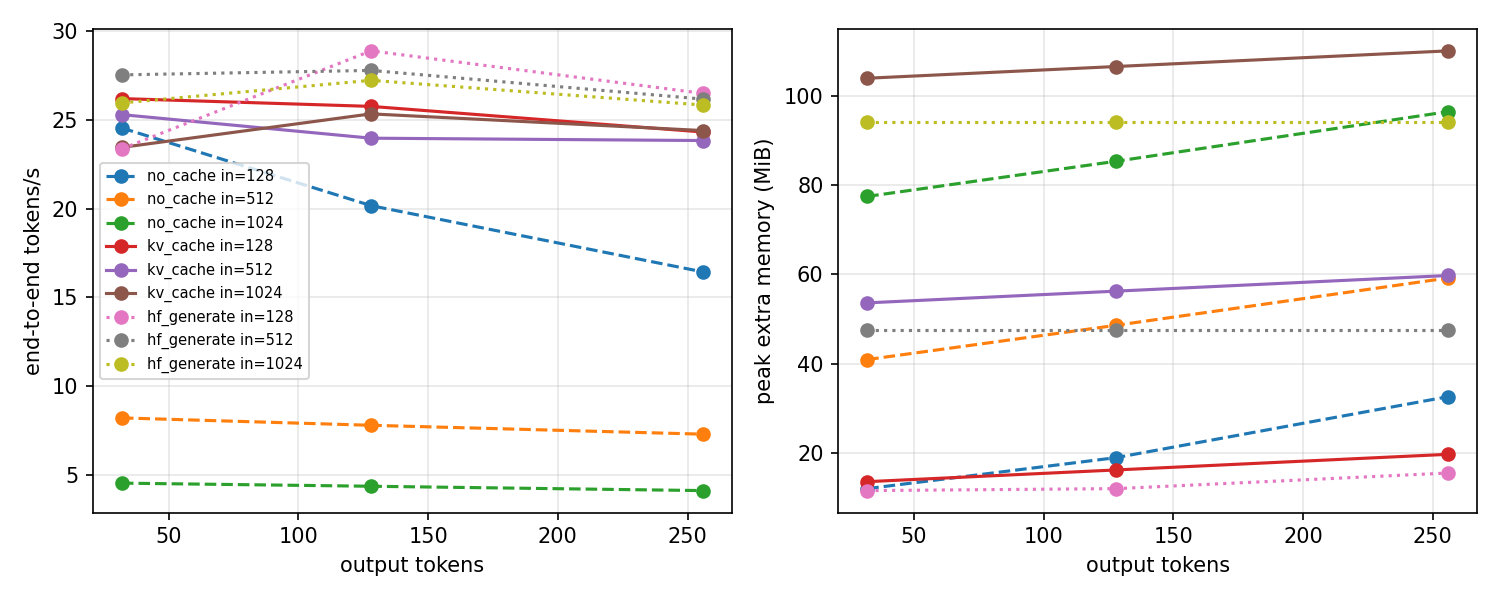
\includegraphics[width=\columnwidth]{kv_bench.png}
\caption{End-to-end throughput and peak extra memory for uncached, KV-cached and library decoding (T4).}
\label{fig:kv}
\end{figure}

\subsection{Tiled Attention}
All 20 controlled cases pass (10 shapes $\times$ fp32/fp16), including non-divisible lengths and block sizes, an unmasked case, cross-length queries, a 33-query chunk continuing after 64 cached keys and a single decode query over 300 keys. The maximum absolute error of the tiled implementation against float64 is $2.3\times10^{-6}$ (mean $\le5.8\times10^{-8}$) in fp32 and $9.7\times10^{-4}$ in fp16, the same as the reference implementation; a case with logits scaled by 30 checks the running-maximum rescaling.

Table~\ref{tab:attn} and Fig.~\ref{fig:attn} compare speed and memory (12 heads, $d{=}128$, causal, fp16). The tiled version reduces peak memory from 2,304\,MiB to 39\,MiB at 4,096 tokens (59$\times$) but is 4.7$\times$ slower than the reference and about 76$\times$ slower than PyTorch's memory-efficient SDPA kernel. An educational PyTorch implementation cannot win on speed: each tile launches several small kernels from a Python loop, and intermediate tiles are written to and read from global memory between kernels, whereas a fused kernel keeps tiles in on-chip SRAM inside a single launch~\cite{flashattn}. The flash backend is unavailable on the T4 (compute capability 7.5; it requires 8.0), which the benchmark records instead of failing.

\begin{table*}[t]
\centering
\caption{Attention implementations on a T4, causal, fp16: time per call (ms) / peak extra memory (MiB), median of 10.}
\label{tab:attn}
\begin{tabular}{lccccc}
\toprule
Implementation & 256 & 512 & 1024 & 2048 & 4096 \\
\midrule
reference (full matrix) & 0.59 / 9 & 1.31 / 36 & 4.49 / 144 & 16.92 / 576 & 66.53 / 2304 \\
tiled online-softmax & 2.59 / 7 & 8.22 / 8 & 27.04 / 12 & 99.77 / 21 & 311.30 / 39 \\
SDPA math backend & 0.55 / 13 & 1.14 / 40 & 3.69 / 137 & 14.08 / 496 & 56.01 / 1888 \\
SDPA memory-efficient backend & 0.09 / 1 & 0.14 / 2 & 0.34 / 3 & 1.09 / 6 & 4.07 / 12 \\
SDPA flash backend & n/a & n/a & n/a & n/a & n/a \\

\bottomrule
\end{tabular}
\end{table*}

\begin{figure}[t]
\centering
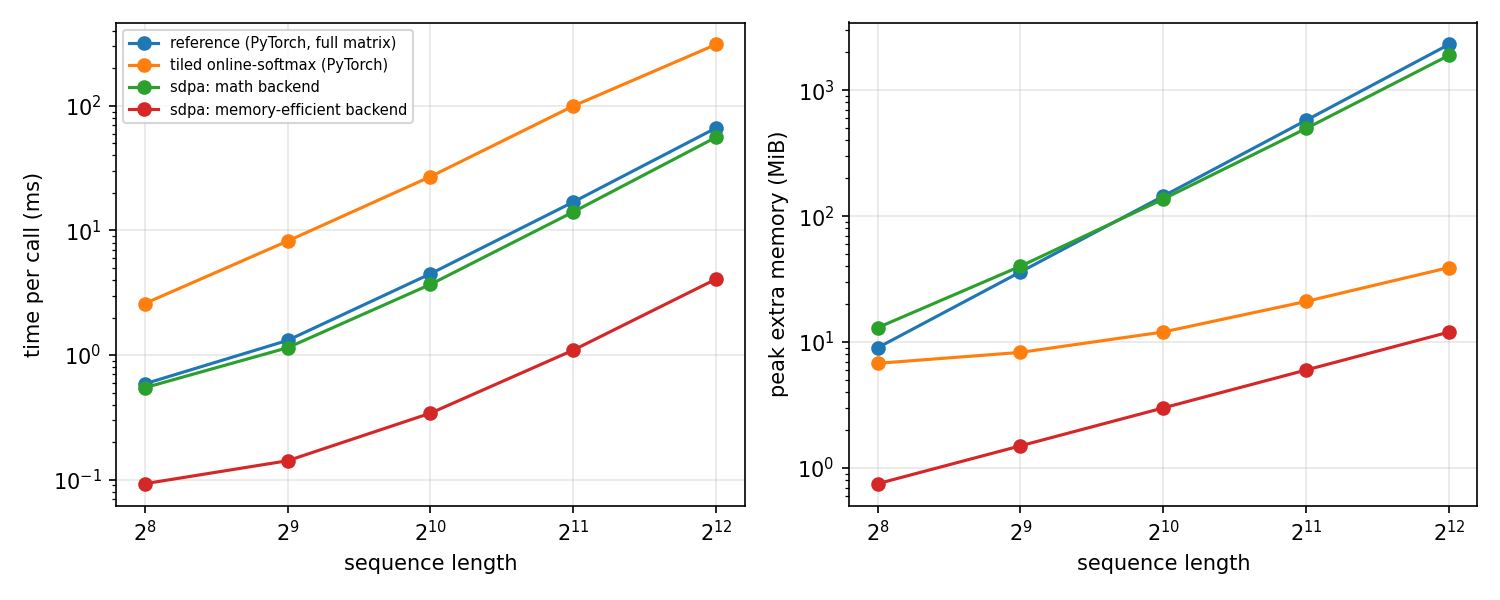
\includegraphics[width=\columnwidth]{attention_bench.png}
\caption{Time and peak memory of the attention implementations versus sequence length (log scales).}
\label{fig:attn}
\end{figure}

\subsection{Speculative Decoding}
Speculative decoding produced exactly the target's greedy tokens in all 240 prompt runs (2 settings, up to 2 drafts, 4 values of $k$, 20 prompts), and Hugging Face assisted generation agreed with greedy on 5 of 5 reference prompts. On CPU we additionally exercised the extremes: a 0\% acceptance draft (every round rejected and corrected) and an identical draft (every round fully accepted with a bonus token), both token-identical.

Table~\ref{tab:spec} and Fig.~\ref{fig:spec} report efficiency. Fine-tuning the draft raises acceptance on screening JSON from 0.66 to 0.96 at $k{=}4$ and cuts target forward passes from 271 to 66 at $k{=}6$. Yet there is no real speed-up: 0.58--0.93$\times$ on screening outputs and at best 1.02$\times$ on 128-token summaries. The reason is measured, not assumed. At batch size 1 on a T4 a forward pass is dominated by per-layer kernel-launch and Python overhead rather than arithmetic, so cost scales with depth more than width: the 24-layer 0.5B draft costs about 26\,ms per token against 40\,ms for the 28-layer target (ratio $c\approx0.65$, not the $\approx0.33$ suggested by parameter counts). With expected accepted length $\frac{1-\alpha^{k+1}}{1-\alpha}$ per round and round cost $(ck+1)$ target steps, even $\alpha=0.96$, $k=4$ predicts at most 1.3$\times$; per-round overheads (two cache crops, Python control flow, host synchronisation for the acceptance test) and the draft's own prefill remove that margin. Screening outputs are only about 15 tokens, so prefill dominates there too. Speculation would help with a much cheaper draft (fewer layers), larger batches, CUDA graphs or a memory-bound target.

\begin{table}[t]
\centering
\caption{Speculative decoding (T4, fp16). A: screening JSON, fine-tuned target, 20 val prompts (greedy 24.9 tok/s). B: free-text summaries, base target (greedy 24.3 tok/s). Fwd = target forward passes, speculative/greedy.}
\label{tab:spec}
\setlength{\tabcolsep}{2pt}
\footnotesize
\begin{tabular}{llccccccc}
\toprule
Set & Draft & $k$ & Acc. & Acc./rd & Fwd & Tok/s & Speed-up & Equal \\
\midrule
A & base & 1 & 0.92 & 0.92 & 153/271 & 23.3 & 0.93$\times$ & 20/20 \\
A & base & 2 & 0.73 & 1.46 & 129/271 & 19.6 & 0.79$\times$ & 20/20 \\
A & base & 4 & 0.66 & 2.64 & 104/271 & 15.8 & 0.64$\times$ & 20/20 \\
A & base & 6 & 0.67 & 4.04 & 88/271 & 14.4 & 0.58$\times$ & 20/20 \\
A & fine-tuned & 1 & 0.98 & 0.98 & 149/271 & 22.8 & 0.92$\times$ & 20/20 \\
A & fine-tuned & 2 & 0.95 & 1.90 & 110/271 & 22.9 & 0.92$\times$ & 20/20 \\
A & fine-tuned & 4 & 0.96 & 3.84 & 82/271 & 20.9 & 0.84$\times$ & 20/20 \\
A & fine-tuned & 6 & 0.93 & 5.59 & 66/271 & 20.2 & 0.81$\times$ & 20/20 \\
B & base & 1 & 0.92 & 0.92 & 1240/2360 & 24.9 & 1.02$\times$ & 20/20 \\
B & base & 2 & 0.92 & 1.83 & 860/2360 & 24.9 & 1.02$\times$ & 20/20 \\
B & base & 4 & 0.87 & 3.48 & 560/2360 & 24.1 & 0.99$\times$ & 20/20 \\
B & base & 6 & 0.76 & 4.55 & 460/2360 & 21.4 & 0.88$\times$ & 20/20 \\

\bottomrule
\end{tabular}
\end{table}

\begin{figure}[t]
\centering
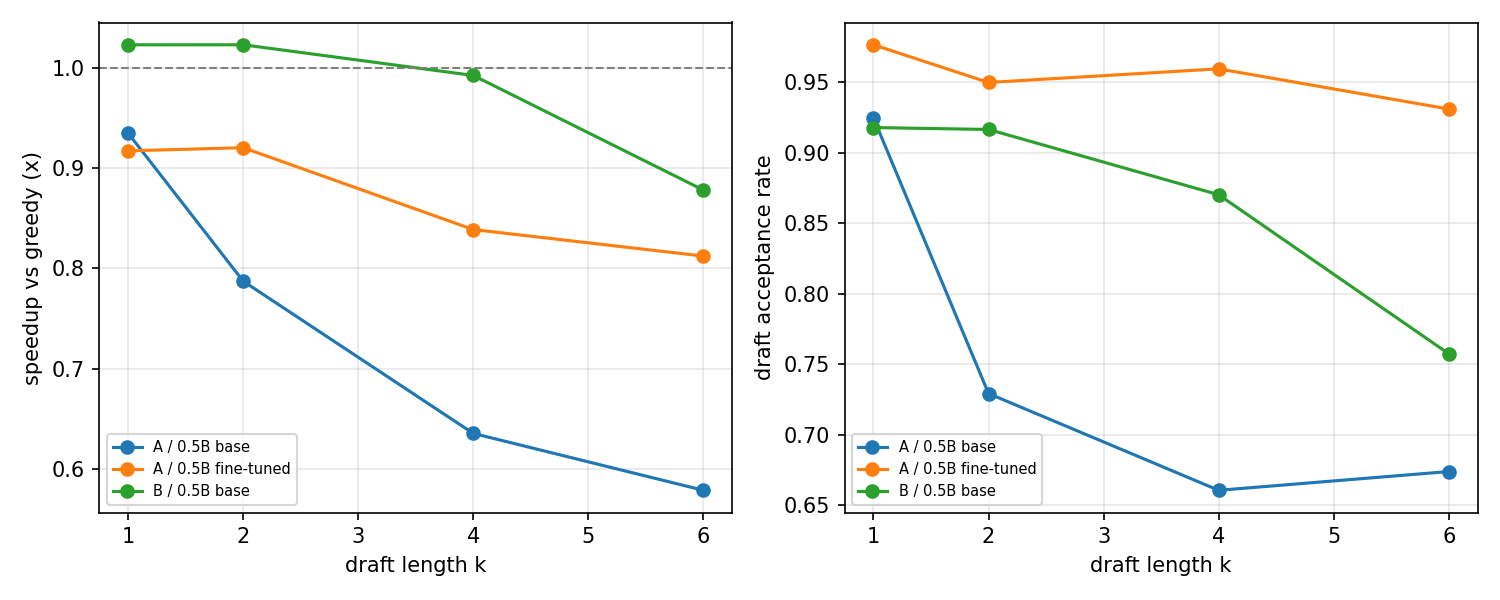
\includegraphics[width=\columnwidth]{spec_bench.png}
\caption{Speed-up over greedy decoding and draft acceptance rate versus draft length $k$.}
\label{fig:spec}
\end{figure}

\subsection{Design Alternatives and Observed Difficulties}
Table~\ref{tab:alternatives} summarises the alternatives we considered and the evidence behind each final choice. Several difficulties shaped the system:
\begin{enumerate}
\item \textbf{Library incompatibility.} Colab's preinstalled \texttt{torchao}~0.10 made PEFT refuse to create LoRA layers; it is uninstalled in every notebook's setup cell.
\item \textbf{API change in Transformers~5.} RoPE settings moved from \texttt{rope\_theta} to \texttt{rope\_parameters}, so our decoder's first configuration check rejected plain RoPE; it now reads both formats.
\item \textbf{Sampling defaults.} Qwen2.5-Instruct ships a generation configuration that samples (temperature 0.7, top-p 0.8, top-k 20, repetition penalty 1.1); setting \texttt{do\_sample=False} alone does not remove the penalty, so we replace the whole configuration for every evaluation.
\item \textbf{Dirty data.} Annotation 883 has an empty criterion and crashed prompt construction; it is dropped and recorded in the manifest.
\item \textbf{CPU memory.} With a browser and IDE open, the laptop could not hold the fp32 model and the app was killed by the out-of-memory killer; precision is now chosen from free memory, and the draft falls back to bf16.
\item \textbf{Free hosting.} Hugging Face no longer hosts Gradio Spaces on the free tier, so the application is run locally with a one-step launcher.
\end{enumerate}

\begin{table}[t]
\centering
\caption{Design alternatives and evidence for the final choice.}
\label{tab:alternatives}
\footnotesize
\begin{tabular}{p{1.55cm}p{1.95cm}p{3.75cm}}
\toprule
Decision & Alternatives & Choice and evidence \\
\midrule
Target & Llama-3.2-1B, SmolLM2-1.7B, Phi-3.5-mini & Qwen2.5-1.5B: Apache-2.0, 2 KV heads, same-tokenizer 0.5B draft, fits T4 (8.5\,GB peak) \\
Adaptation & full fine-tuning, QLoRA & LoRA $r{=}16$ on all projections: 1.2\% trainable, no quantisation error \\
Loss & full sequence & answer tokens only (prompt masked) \\
Checkpoint & last step & lowest validation loss (step 50; loss rises after) \\
Imbalance & oversampling & rejected: rare-label F1 still 0, evidence F1 $-$0.07 (Table~\ref{tab:design}) \\
Explanation & free-text generation & template from cited sentences (no supervision allowed; cannot invent facts) \\
Output order & label first & evidence first, so the label is conditioned on the citations (not ablated) \\
Decoding & library defaults & explicit greedy, repetition penalty 1.0 \\
Draft & base 0.5B & fine-tuned 0.5B: acceptance 0.66$\rightarrow$0.96 ($k{=}4$) \\
Attention mask & \texttt{is\_causal=True} & explicit offset mask (correct for cached chunks) \\
App precision & bf16 on CPU & fp32 when memory allows (bf16 2.7$\times$ slower on AVX2) \\
\bottomrule
\end{tabular}
\end{table}

\subsection{Computational Resources}
Each fine-tuning run took 16.3 minutes on a free T4 with a peak of 8.5\,GB; evaluating 206 criteria takes 22--34\,s. All benchmarks fit in the T4's 15\,GB. On a 15\,GB-RAM laptop CPU, the 1.5B model needs about 6.2\,GB in fp32; with a browser and IDE open, only bf16 fitted, and bf16 was 2.7$\times$ slower than fp32 on this AVX2 CPU (no native bf16 matrix units), so the application chooses the precision from available memory and loads the draft in bf16 when memory is tight (the output stays identical because the target verifies every token).

% =====================================================================
\section{Limitations}
(1) The training set has 37 patients and 602 criteria from short TREC-style case reports; real notes are longer and noisier, and the 8-patient test set gives wide confidence intervals (test accuracy 0.55--0.81). (2) The model never predicts \emph{not applicable}, \emph{not included} or \emph{excluded} on test, and on exclusion criteria it does not beat the majority baseline. (3) It reproduces the annotators' tendency to treat unmentioned exclusion conditions as absent; we flag such decisions as unsupported rather than correct them. (4) Explanations are templates, not generated reasoning; they are faithful to the cited evidence but shallow. (5) The rule-based overall outcome is not validated against any patient-level ground truth. (6) Our speculative decoder is slower than greedy decoding in every measured setting at batch size 1. (7) The system is a research screening prototype and must not be used for enrolment decisions.

\section{Conclusion}
A 1.5B open model fine-tuned with LoRA on 602 criteria raises held-out accuracy from 0.18 to 0.69 and evidence F1 from 0.22 to 0.51, runs on free hardware, and cites the sentences behind each decision. Its errors are interpretable: missing information treated as absence, failed numeric or clinical inference, and ambiguous applicability labels. The hand-written KV cache, tiled attention and speculative decoder are verified token-for-token or to $10^{-6}$ against references; the cache gives up to 5.9$\times$ (GPU) and 9.4$\times$ (CPU) speed-ups, tiled attention gives a 59$\times$ memory reduction, and speculative decoding is correct but slower here for reasons we quantified. Future work: class-weighted training for rare labels, explicit numeric-threshold checking, and a shallower draft model.

\appendices
\section{Reproducibility}
\begin{itemize}
\item \textbf{Source code, split manifest, logs and results:} \url{https://github.com/FatimaRana50/Trialmatch} (\texttt{data/split\_manifest.json}, \texttt{results/}, \texttt{logs/}, \texttt{requirements.txt}).
\item \textbf{Target adapter (Qwen2.5-1.5B + LoRA):} \url{https://huggingface.co/f777777777/trialmatch-qwen2.5-1.5b-lora}
\item \textbf{Draft adapter (Qwen2.5-0.5B + LoRA):} \url{https://huggingface.co/f777777777/trialmatch-qwen2.5-0.5b-draft-lora}
\item \textbf{Demonstration video:} \url{https://youtu.be/EhLhlF_ktfA}
\item \textbf{Experiments:} run notebooks 01--06 in \texttt{notebooks/} on a free Colab T4 (01 split, 02 baseline and fine-tuning, 02b oversampling, 03 single final test, 04 KV cache and attention, 05 speculative decoding, 06 weight upload). Every table in this paper is regenerated by \texttt{src/make\_report\_tables.py} and \texttt{src/extra\_analysis.py}.
\item \textbf{Application:} run \texttt{./run\_app.sh} (Linux/macOS) or \texttt{run\_app.bat} (Windows); it creates a virtual environment, downloads the weights and opens \texttt{http://127.0.0.1:7860}.
\end{itemize}

\section{AI-Use Statement}
An AI coding assistant (Anthropic Claude, used through Claude Code in VS Code) was used to help write and debug the data pipeline, training and evaluation scripts, the decoder, attention and speculative-decoding implementations, the application and the first draft of this report. All code was run and tested by the author: unit and equivalence tests (cached vs.\ uncached tokens, tiled vs.\ float64 attention, speculative vs.\ greedy tokens, shared-prefix reuse vs.\ fresh decoding) were executed, every number in this paper is generated from the result files in the repository by \texttt{src/make\_report\_tables.py}, and the author reviewed and can explain each component. The TrialGPT repository was consulted only as a reference; no TrialGPT outputs were used.

\begin{thebibliography}{99}
\bibitem{trialgpt} Q.~Jin, Z.~Wang, C.~S.~Floudas, F.~Chen, C.~Gong, D.~Bracken-Clarke, E.~Xue, Y.~Yang, J.~Sun, and Z.~Lu, ``Matching patients to clinical trials with large language models,'' \emph{Nature Communications}, vol.~15, art.~9074, 2024.
\bibitem{trialgptdata} NCBI, ``TrialGPT-Criterion-Annotations,'' Hugging Face dataset, \url{https://huggingface.co/datasets/ncbi/TrialGPT-Criterion-Annotations}.
\bibitem{koopman} B.~Koopman and G.~Zuccon, ``A test collection for matching patients to clinical trials,'' in \emph{Proc.\ ACM SIGIR}, 2016, pp.~669--672.
\bibitem{criteria2query} C.~Yuan, P.~B.~Ryan, C.~Ta, Y.~Guo, Z.~Li, J.~Hardin, R.~Makadia, P.~Jin, N.~Shang, T.~Kang, and C.~Weng, ``Criteria2Query: a natural language interface to clinical databases for cohort definition,'' \emph{J.\ Am.\ Med.\ Inform.\ Assoc.}, vol.~26, no.~4, pp.~294--305, 2019.
\bibitem{vaswani} A.~Vaswani \emph{et al.}, ``Attention is all you need,'' in \emph{Proc.\ NeurIPS}, 2017, pp.~5998--6008.
\bibitem{qwen25} Qwen Team, ``Qwen2.5 technical report,'' arXiv:2412.15115, 2024.
\bibitem{rope} J.~Su, M.~Ahmed, Y.~Lu, S.~Pan, W.~Bo, and Y.~Liu, ``RoFormer: Enhanced transformer with rotary position embedding,'' \emph{Neurocomputing}, vol.~568, 2024.
\bibitem{gqa} J.~Ainslie, J.~Lee-Thorp, M.~de~Jong, Y.~Zemlyanskiy, F.~Lebr\'on, and S.~Sanghai, ``GQA: Training generalized multi-query transformer models from multi-head checkpoints,'' in \emph{Proc.\ EMNLP}, 2023.
\bibitem{lora} E.~J.~Hu \emph{et al.}, ``LoRA: Low-rank adaptation of large language models,'' in \emph{Proc.\ ICLR}, 2022.
\bibitem{adamw} I.~Loshchilov and F.~Hutter, ``Decoupled weight decay regularization,'' in \emph{Proc.\ ICLR}, 2019.
\bibitem{qlora} T.~Dettmers, A.~Pagnoni, A.~Holtzman, and L.~Zettlemoyer, ``QLoRA: Efficient finetuning of quantized LLMs,'' in \emph{Proc.\ NeurIPS}, 2023.
\bibitem{mqa} N.~Shazeer, ``Fast transformer decoding: One write-head is all you need,'' arXiv:1911.02150, 2019.
\bibitem{pope} R.~Pope \emph{et al.}, ``Efficiently scaling transformer inference,'' in \emph{Proc.\ MLSys}, 2023.
\bibitem{vllm} W.~Kwon \emph{et al.}, ``Efficient memory management for large language model serving with PagedAttention,'' in \emph{Proc.\ ACM SOSP}, 2023.
\bibitem{flashattn} T.~Dao, D.~Y.~Fu, S.~Ermon, A.~Rudra, and C.~R\'e, ``FlashAttention: Fast and memory-efficient exact attention with IO-awareness,'' in \emph{Proc.\ NeurIPS}, 2022.
\bibitem{rabe} M.~N.~Rabe and C.~Staats, ``Self-attention does not need $O(n^2)$ memory,'' arXiv:2112.05682, 2021.
\bibitem{onlinesoftmax} M.~Milakov and N.~Gimelshein, ``Online normalizer calculation for softmax,'' arXiv:1805.02867, 2018.
\bibitem{leviathan} Y.~Leviathan, M.~Kalman, and Y.~Matias, ``Fast inference from transformers via speculative decoding,'' in \emph{Proc.\ ICML}, 2023.
\bibitem{chen} C.~Chen, S.~Borgeaud, G.~Irving, J.-B.~Lespiau, L.~Sifre, and J.~Jumper, ``Accelerating large language model decoding with speculative sampling,'' arXiv:2302.01318, 2023.
\bibitem{hftransformers} T.~Wolf \emph{et al.}, ``Transformers: State-of-the-art natural language processing,'' in \emph{Proc.\ EMNLP: System Demonstrations}, 2020, pp.~38--45.
\end{thebibliography}

\end{document}
